%\documentclass[prodmode,acmtecs]{acmconf} % Aptara syntax
\documentclass{sig-alternate}
\usepackage{url}
\usepackage{graphicx}
\usepackage{amsmath}
\usepackage{color}
\usepackage{multirow}
\usepackage[ruled]{algorithm2e}

\newcommand{\sui}[1]{%
  \textcolor{green}{SC - #1}
}

\newcommand{\marc}[1]{%
  \textcolor{red}{[MC: #1]}
}

\newcommand{\greg}[1]{%
  \textcolor{blue}{GB: #1}
}

%\ConferenceShortName{ICS}
%\ConferenceName{International Conference on Supercomputing}

\title{Comprehensive Algorithmic Resilience for Scientific Applications}
\author{Sui Chen, 
%\affil{Louisiana State University}
Greg Bronevetsky, Marc Casas-Guix
%\affil{Lawrence Livermore National Laboratory}
Lu Peng,
%\affil{Louisiana State University}
}

\begin{document}

\maketitle

\begin{abstract}
As High-Performance Computing (HPC) systems become larger and more complex and the feature sizes of their electronic components grow smaller, the systems become increasingly vulnerable to soft faults.
Since such faults may cause application crashes or may silently corrupt application results it is necessary to develop techniques to protect applications from such errors at a low cost in performance and power.
Despite extensive work on general-purpose resilience techniques, they are cost effective for protecting only certain system components, such as memories.
To provide comprehensive protection for the computations of HPC applications it is necessary to develop algorithmic resilience mechanisms that use the properties of algorithms to provide cost-effective protection.

Algorithmic resilience can be very complex to deploy in applications because a comprehensive resilience strategy must address all the types of errors that an application may experience.
This includes corruptions to numerical data as well as control information and data structures.
Full protection requires the combination of multiple techniques including algorithmic error detection, crash detection, replication of key control information as well as support for restart when errors are detected.
Further, it is necessary to configure the properties of the resilience mechanisms to make sure that they are cost-effectively meeting the user's accuracy and confidence targets.
This paper shows how all these issues can be resolved comprehensively in the context of three numeric applications.

\end{abstract}

\section{Introduction}
\label{sec:intro}

The increasing size and complexity of HPC systems is making them increasingly vulnerable to soft faults.
Soft faults are transient corruptions of circuit state caused by physical phenomena such as strikes by neutrons or alpha particles~\cite{baumann:2005, asciQSER:2005} or thermal electrical noise~\cite{therm_noise:2007}.
They can affect the state of processor latches and registers and may cause the application to crash or worse, to silently return incorrect results~\cite{mpi_ser:reed:2004}.
As the electronic feature sizes shrink technology scaling will make soft errors a larger problem~\cite{err_scaling:2012} due to the fact that each circuit element will hold less charge and can thus be disrupted by easily.
These phenomena make it imperative to develop techniques to make HPC systems resilient to soft faults.

Resilience is a problem that must be addressed at all levels.
While materials science and circuit design techniques can be used to improve resilience, they come at a cost in reduced power efficiency and performance that an become prohibitive if processors need to be sufficiently reliable to build a large HPC system.
Techniques such as error correcting codes have been very effective at making memories and caches resilient to soft faults~\cite{mem_errors:2010}.
However, they are more expensive for protecting core-internal state such as latches and are significantly less effective for checking the correctness of computations.
Traditional approaches like cross-core or node replication~\cite{rmpi:2011, dyn_cmp_repl:2007} are expensive in their use of computing resources and power and their long error detection latencies require processor state to be frequently checkpointed.
Processor designs that incorporate instruction replication~\cite{repl_smt:2000} offer fine-grained error detection and rollback but require more power as well as novel hardware features that are not likely to be included in the commodity processors must be used in HPC systems to limit their cost.

The limitations of automated resilience techniques has motivated the need for algorithmic techniques that can detect and tolerate errors by taking advantage of application-specific properties and invariants~\cite{amg_abft:2012, robustification:2010, abft:1984}.
Although these techniques can be very efficient most research work on such techniques has primarily focused on their algorithmic properties and how they can be leveraged to enable accurate error detection.
While this goal is important, it ignores the full complexity of the problem since it focuses narrowly on errors in numeric data while ignoring errors in control information and data structures.
In reality a comprehensive solution must incorporate a range of additional techniques such as key variable replication, memory violation detection and localized rollback on detected error, as well as techniques to configure these various resilience methods to achieve the best performance given the user's accuracy and confidence targets.
%, they also require manual effort to incorporate into applications and may require deep insight into an application's invariants to deploy effectively.
%Fortunately, because real-world applications spend most of their execution is spent in a few application modules, most soft faults will occur in those modules rather than uniformly throughout the application.
%In scientific applications these modules are usually various types of libraries, including numeric solvers and domain-specific scientific packages.
%This indicates that if by focusing algorithmic resilience efforts on the key library routines, while leaving other modules unprotected or protected via more expensive mechanisms, it is possible to fully protect an application at a low cost.

This paper presents a comprehensive algorithmic resilience approach that considers all of the above issues.
We demonstrate it on different types of numerical applications: the Alternating Direction Method of Multipliers (ADDR) for Lasso problems~\cite{lasso:2011}, the Hattrick gravitational simulation~\cite{hattrick:2012} and the Digital Room Correction (DRC) acoustic correction application~\cite{drc:2012}.
We show how these three applications can be comprehensively protected from soft faults by adding three different resilience mechanisms to the routines where they spend the most time: algorithmic error checks, replication of critical data structures and checkpoint-restart of individual routines.
We demonstrate via fault injection experiments that although none of these techniques can individually protect applications from soft faults, their combination is highly effective.
Further, we demonstrate how these techniques can be parameterized to offer the right level of protection at any given fault rate or input type, and further can be tuned to bound the probability that the application will produce erroneous results or executes for longer than some limit.

\section{Soft Faults}
\label{sec:soft_faults}

Causes of soft faults and how they manifest themselves in applications.

Discuss prior work on replication and algorithmic techniques, emphasize that in this paper we're focusing on software resilience since hardware resilience is extremely difficult to deploy in real processors since the costs have to be carried by non-HPC markets that care much less about it.

Can show plots of how routine results are affected by injected errors. Should show this for all the routines we'll be considering in this paper.

Describe fault injection framework and how it approximates real faults.

\section{Target Applications}
\label{sec:apps}

We evaluate our library-based resilience approach by applying it to the following three applications.
As they make intensive use library routines, they are ideal testbeds for our proposed fault-tolerance methods.

\greg{This section needs to include an experimental breakdown of where the routines spent their time. We also need to describe the types of inputs we'll be giving them in our experiments.}

\subsection{Alternating Direction Method of Multipliers (ADDR)}
\label{sec:apps:lasso}
The ADDR method solves under-unconstrained linear problems $Ax=b$ for $x$ ($A$ has fewer rows than columns) while minimizing the function $f(x)$.
This is an iterative algorithm that spends most of its time in the linear algebra operations, matrix-matrix multiplication, matrix-vector multiplication, rank-k update and Cholesky factorization, using the implementations of these routines from the GNU Scientific Library~\cite{gsl:2011}.
We focused on a specific application that uses the ADDR method to solve Lasso problems, which are defined as minimizing the function $\frac{1}{2} \left|| Ax - b \right||_2^2 + \lambda*\left|| x \right||_1$.
In our experiments we considered linear systems of size \textbf{???} that were generated \textbf{???}.

\subsection{DRC: Digital Room Correction}
\label{sec:apps:drc}

The DRC program generates filters for HiFi audio systems to compensate for the reflection of sounds in a room, using impulse response measurements of the audio equipment and considering the positions of the listeners.
Although the algorithm is divided into many phases the most computationally intensive step consists of the GSL's implementation of the Fast Fourier Transform.
\greg{What inputs?}

\subsection{Hattrick}
\label{sec:apps:hattrick}
The Hattrick application simulates the motion of bodies under the effects of gravity.
It is designed to help discover extra-solar planets by inferring their existence from Transit Timing Variations, where the difference between the times when a planet passes in front of its host star is used to infer the existence and properties of other planets in the system.
This program spends most of its execution time in the GSL solver for Ordinary Differential Equations to solver the system's equations of motion.

\section{Resilience Techniques}
\label{sec:res_tech}

\subsection{Error Detection}
\label{sec:res_tech:err_det}

\subsubsection{Algorithmic Detection}
\label{sec:res_tech:err_det:algo}

%\sui{Performance experiments inserted here: running algorithmic checkers across different input sizes and fault rates: 62x62 to 500x500 matrixes for MM, RK, CD, MV checkers; FFT sizes of $2^8$ to $2^{24}$ for the FFT checker; Error bars should apply here, especially for the Cholesky Decomposition checker}

Each algorithm used by the above application was enhanced with an algorithm-specific checker that validated its results by exploiting some algorithmic identity.
Each checker computes some aggregate property of the algorithm's results using two different algorithm to produce vectors $v$ and $v'$ and their relative difference by more than some threshold $\tau$, the checker declares that an error has occurred.
The relative difference is computed as $\frac{\left|| v-v' \right||}{max(\left||v\right||, \left||v'\right||)}$ ???.

\paragraph{Matrix-matrix multiplication (MMM)}:
The MMM operation $A \cdot B$ is checked using a matrix vector multiplication (MVM), making use of this identity: $(A \cdot B) \cdot x = A \cdot (B \cdot x)$, where $x$ is an error-checking vector.
This check is efficient because the checker is asymptotically faster than the MMM algorithm, with MVM taking $O(n^2)$ time and MMM $O(n^3)$ time.
Since we make no assumptions about the distribution of data in the matrixes being multiplied, we set the check vector $x$ to contain all 1's.

\paragraph{Matrix-vector multiplication (MVM)}:
The MVM algorithm $Ax=b$ is checked using a similar identity $(x^TA)x = x^T(Ax) = x^Tb$.
The product $x^TA$ is a checksum of the columns of matrix $A$ and when $x$ is the vector of 1's, the value used in our experiments, it is the sum of $A$'s columns.
Although the computation of $x^TA$ involves additions rather than multiplications the complexity of computing $x^TA$ is $O(n^2)$, the same as the original MVM operation, making this check significantly less efficient.
While this cost can be reduced significantly by computing $x^TA$ once and reusing it in subsequent multiplications by the same matrix, we did not consider it in this paper because MVM took up little application execution time.

\greg{If MVM doesn't matter then why did we protect it? Also, why is the overhead >100\%? Where is the time spent?}

\paragraph{Symmetric Rank-K update (SYRK)}:
The SYRK update is a special case of matrix-matrix multiplication $C = \alpha A \cdot A^T + \beta*C$, where an $nxk$ matrix $A$ is multiplied by itself to produce an $nxn$ matrix with rank $k$, which is added to the $nxn$ matrix $C$.
By decomposing the upper/lower half of the output matrix as a series of sub-matrices (like the sub-cells in a quad tree), the checker takes $O(n^2 \cdot \log{n})$ time, while the original routine takes $O(n^3)$ time.

\paragraph{Cholesky Decomposition (CD)}:
In this decomposition matrix $A$ is decomposed into $L \cdot L^T$ where $L$ is a lower-triangular matrix with a positive diagonal.
This routine is checked just like MMM by checking the identity $Ac = L \cdot (L^T x)$ where $x$ is the vector of all 1's.
This check runs in time $O(n^2)$ while the deterministic CD algorithm has $O(n^3)$ complexity.
The GSL implements an iterative algorithm that runs faster than $O(n^3)$ time but as shown in the experiments below it is significantly slower than our checker.

\paragraph{Fast Fourier Transform (FFT)}:
The FFT algorithm decomposes a function into a sum of sine waves of different frequencies: $f(x) = \sum_{n=0}^{N-1} x_n e^{-i2\pi k n / N}$ for some constant $k$.
We check the results of FFT by using Parseval's theorem, which states that $\sum_{n=0}^{N-1} \left| x[n] \right|^2 = \frac{1}{N} \sum_{k=0}^{N-1} \left| X[k] \right|^2$, where $x$ is the original function and $X$ is its transform.
This means that the total energy of the original function is preserved by the transform and provides an $O(n)$ time check for the $O(n log(n))$ FFT algorithm.

\paragraph{Runge-Kutta PDE Solver (RK)}:
This algorithm uses the \sui{4-th order} Runge-Kutta method for solving Ordinary Differential Equations of the form $\frac{dy}{dx} = f(y, x)$.
It works by advancing the variable $x$ by steps of size $h$ and using estimates of the derivative $\frac{dy}{dx}$ at each point $x$ to find the value of $y$ at the next point $x+h$.
The RK method in GSL uses adaptive step-size control where it simultaneously performs the RK method with two step sizes $h$ and $\frac{h}{2}$ (more precise).
If the difference between the results obtained with the two step sizes are larger than a threshold, the algorithm switches to the smaller step size to maintain accuracy and resumes.
Since the adaptive step control algorithm can also detect errors we utilize it to this end in our work.

\begin{figure}[ht!]
%\vspace{-20pt}
\centering
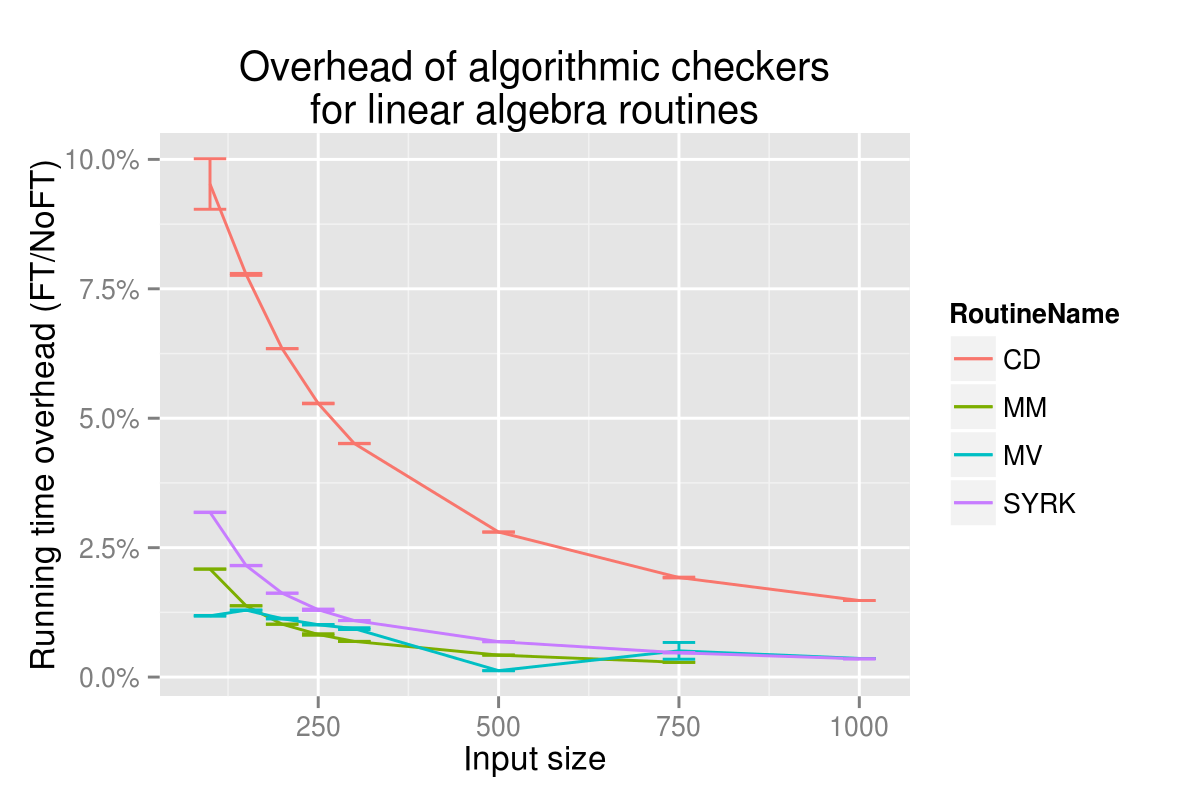
\includegraphics[width=1.00\columnwidth]{figs/4_1_1_Exp1_linalg}
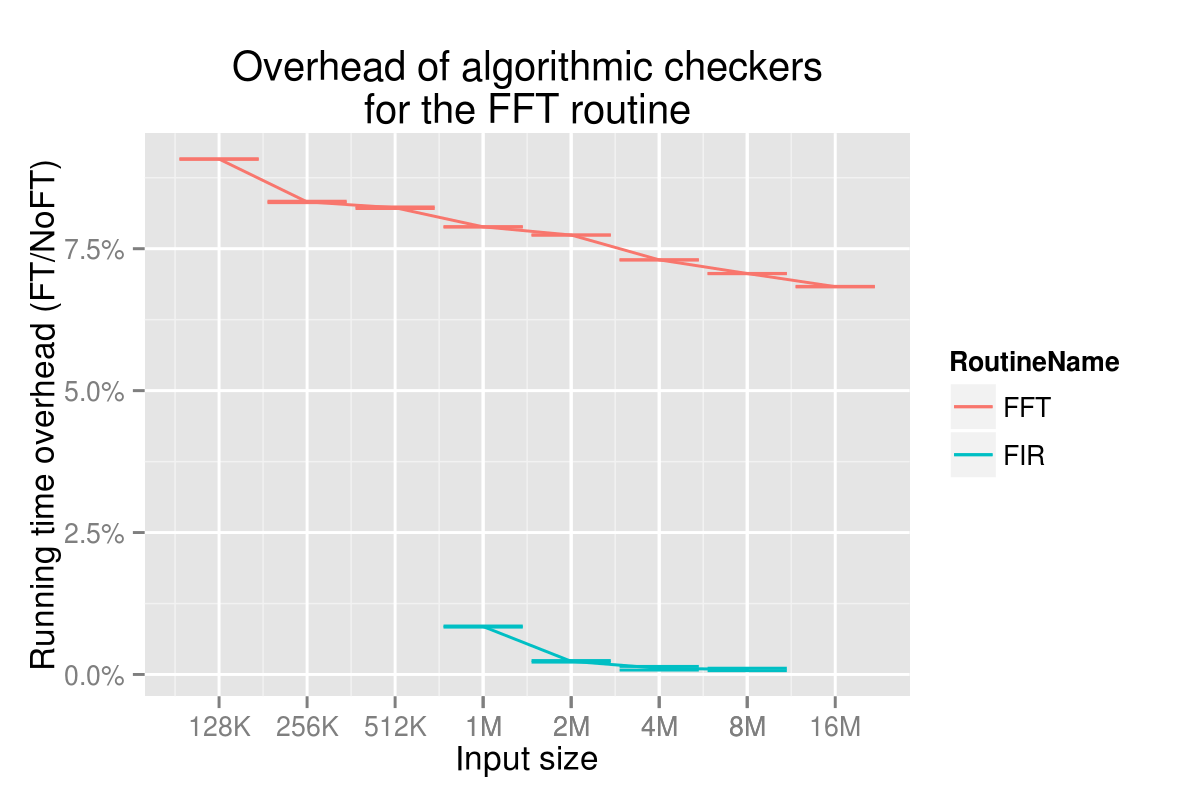
\includegraphics[width=1.00\columnwidth]{figs/4_1_1_Exp1_fft}
%\vspace{-5pt}
\caption{Overhead of the algorithmic resilience techniques of key application routines}
\label{fig:algo_ovhd}
\end{figure}

\begin{figure}[ht!]
\centering
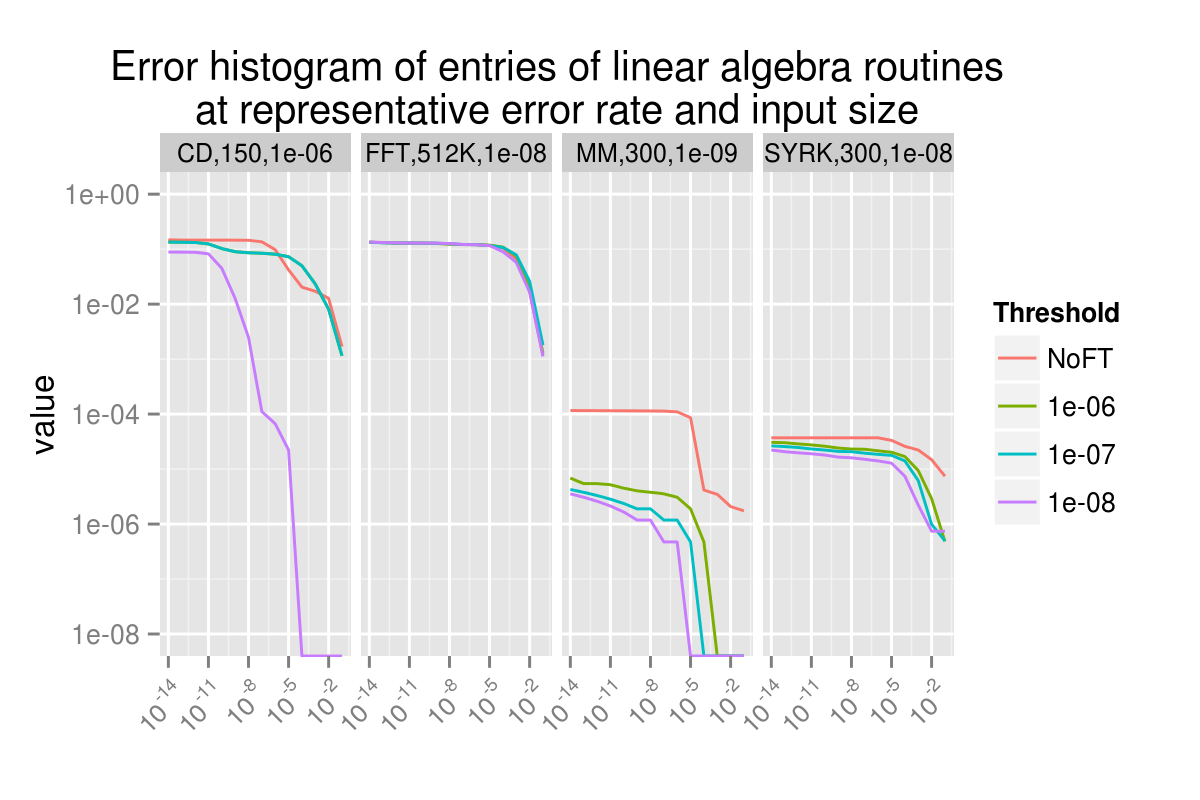
\includegraphics[width=1.00\columnwidth]{figs/4_1_1_Exp2_1_Example.png}
\caption{Error magnitude histogram of one routine}
\end{figure}

\begin{figure}[ht!]
\centering
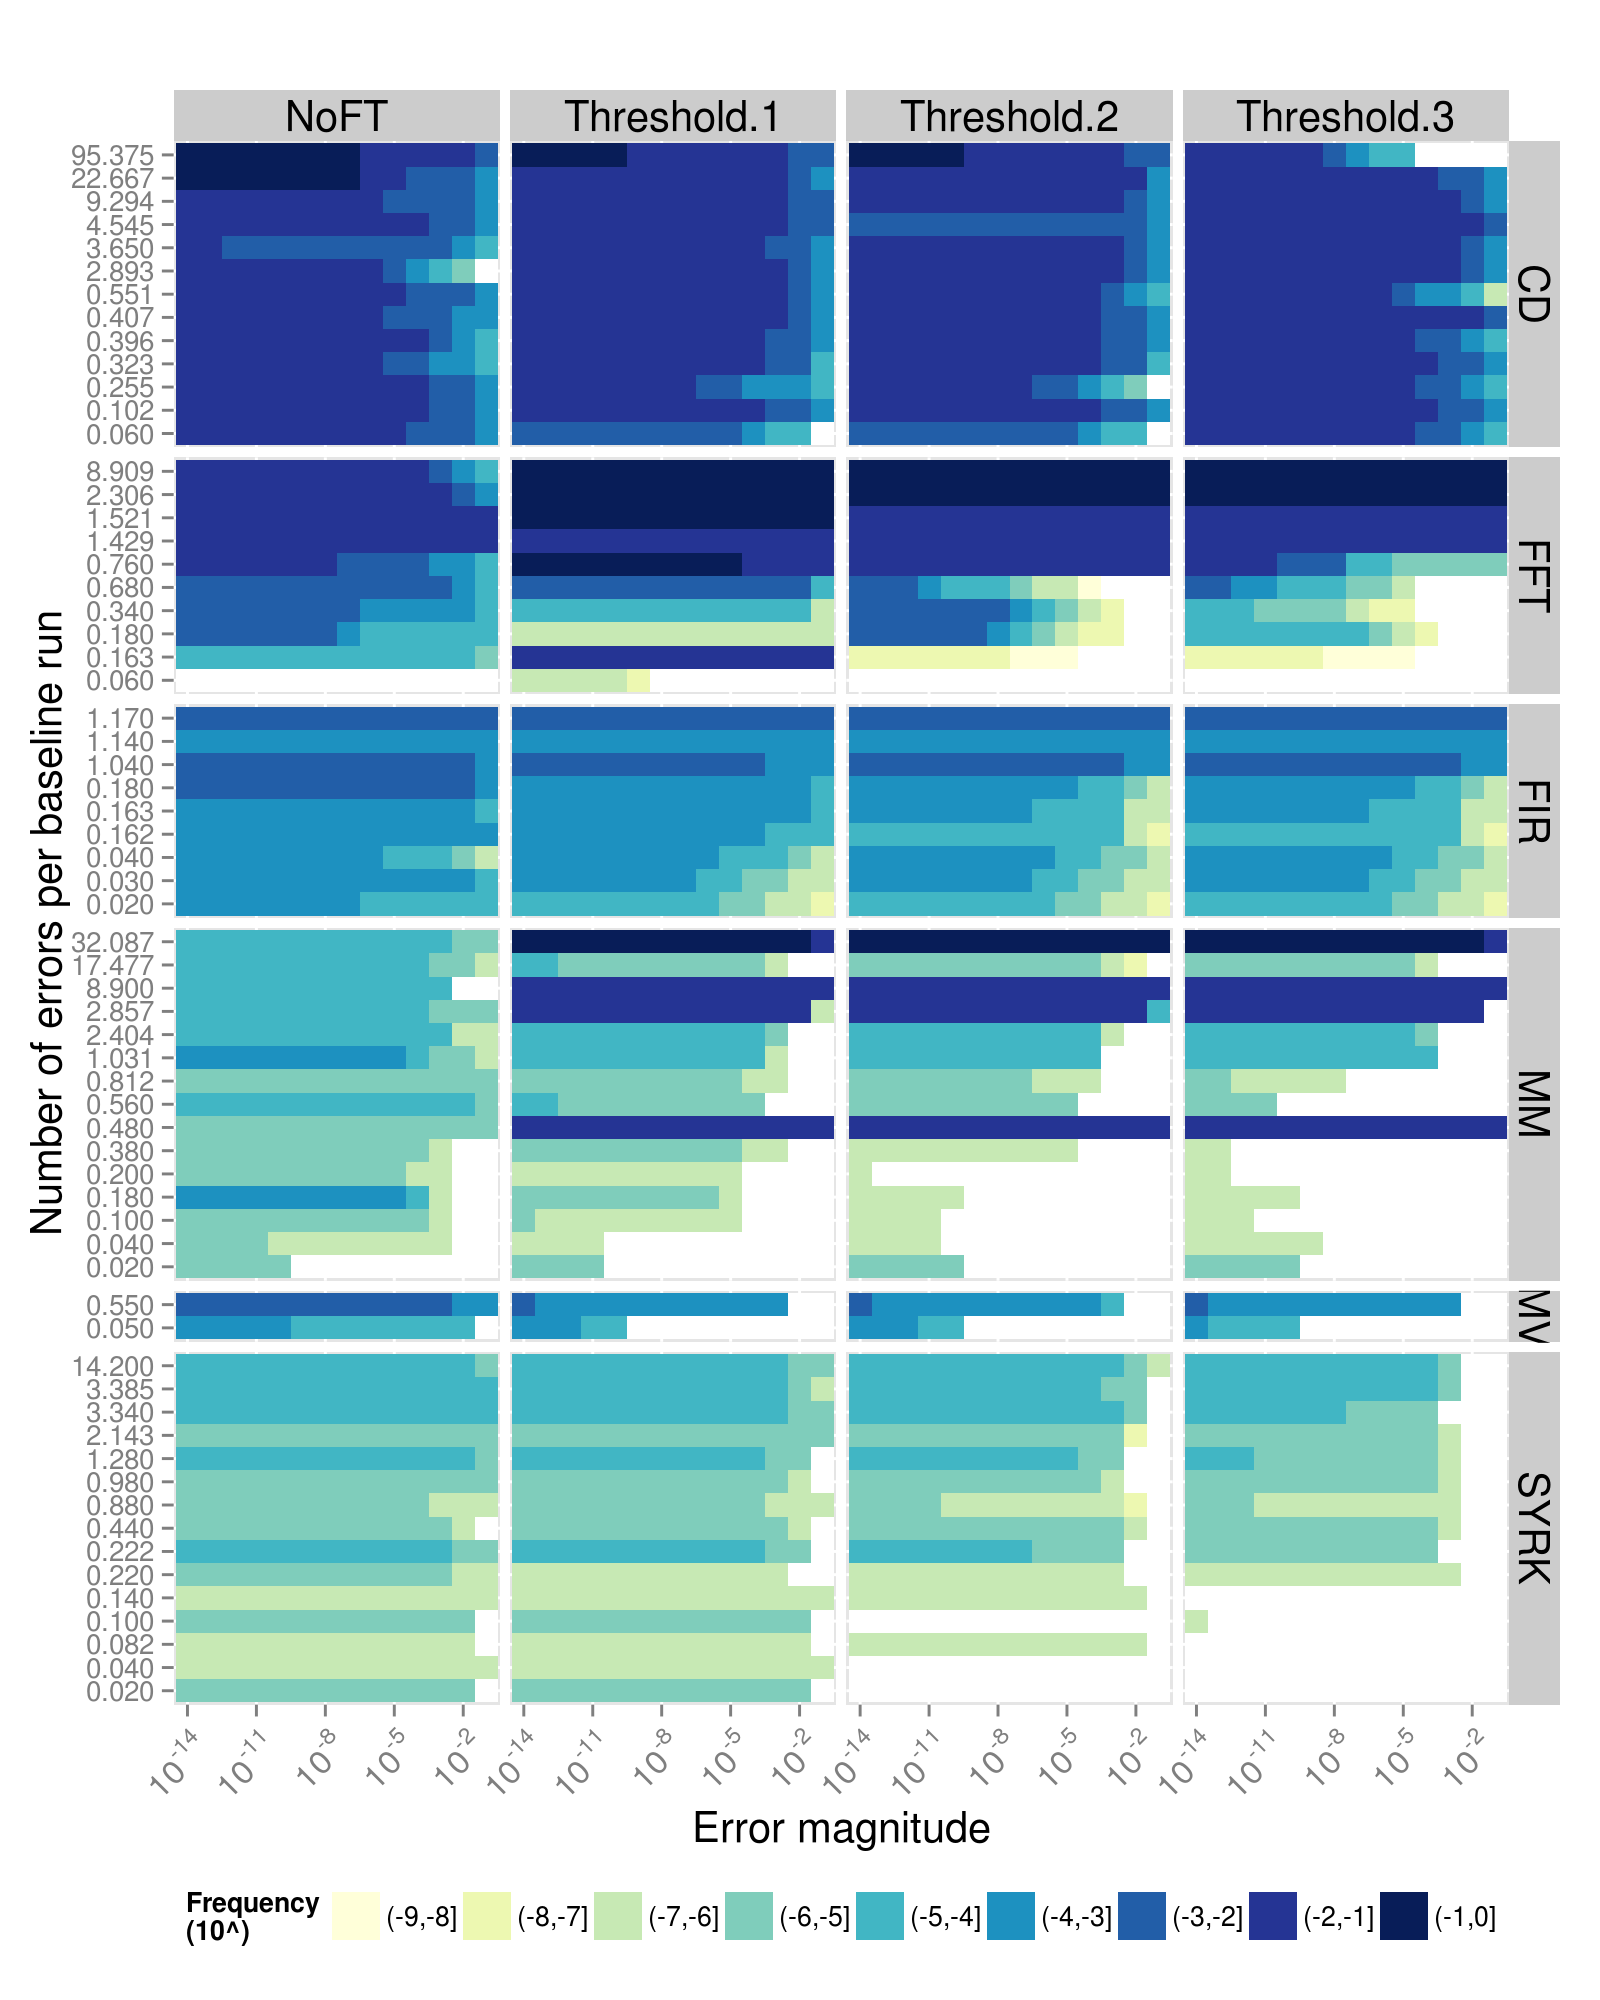
\includegraphics[width=1.00\columnwidth]{figs/4_1_1_Exp2_2_Heatmap_Error_ConfSpace.png}
\caption{Error magnitude histogram of the entire configuration space}
\end{figure}



%Experiment 1: Measure performance degradation of using error detectors as input sizes increase. In case of RK if we can run a version that doesn't do the multiple step sizes, do so but if this is difficult then don't worry about it.
We evaluate the costs of the above algorithmic error checkers by measuring their costs and effectiveness when running at different error rates on different types of inputs.
Figure \ref{fig:algo_ovhd} measures the overheads of employing the checkers in each algorithms when no errors are injected.
The linear algebra routines were executed on $nxn$ square matrixes where $n=(62, 250, 500, 750\ and\ 1000)$.
FFT ran on inputs upto 4M and RK ran on an integral with different intervals $[t_0, t_1]$ where $t_0=0$ and $t_1 \in \{10, 15, 20, 25, 30, 50, 75, 100\}$.
Our experiments show ???\sui{the effectiveness of the error handlers and the error checkers. Note that the graph shows fault injection experiments at various rates (defined by errors per run).}

%Experiment 2: Measure the error in the outputs of the algorithms with and without the algorithmic detectors.
%First, show a probability distribution histogram for all the codes at one error rate, input size and algorithmic detection threshold.
%Then show a summary of the entire space using the same heatmaps that we're using for final application results.
%Put the input size and error rate on the y-axis and the detection threshold on the x-axis.
%The color in each box should be the fraction of entries in the output that have an error of a given magnitude.
%Show a separate plot for a few different magnitudes.

We now evaluate the effectiveness of our algorithmic detectors when errors are injected.
Figure~\ref{fig:algo_err_dist} shows the fraction of entries in the outputs of each routine (y-axis) that have an error of a given magnitude (x-axis) as error magnitudes span from ??? to ??? and errors are injected at rate ???.
In this experiment the liner algebra operations were run on matrixes of size ???, FFT on ??? and RK on ???.
We show results for both the routines with no error checkers as well as routines where error checkers are used with detection thresholds ???.
The data shows ???.

Figure~\ref{fig:algo_err_heatmap} shows the same information across the entire experimental space.
The y-axis includes all algorithms, input sizes and error rates.
The x-axis includes several segments for different degrees of error checking: none, as well as checking with thresholds ???. In each segment the x-axis spans over error magnitudes from ??? to ???.
The box associated with each combination of the four parameters the figure indicates the fraction of outputs that have an error of this magnitude by the shade of gray it is colored with, as indicated in the legend.
The data shows ???

%Experiment 3: Measure the fraction fraction of routine runs that are interrupted by the detection of an error.
%Display this information via the same heatmaps as above.

Finally, Figure~\ref{fig:algor_term_heatmap} shows the fraction of algorithm runs during which the error checks detect errors, across all the algorithms, input sizes, error rates and detection types.
This information is shown in the same format as Figure~\ref{fig:algo_err_heatmap} and is important for informing us about the performance impact of error detection at these error rates since each error detection results in a rollback of application execution.
The experiments show ???.

\greg{For each experiment we need to include a discussion of what it means for how these checkers behave within the full-application runs.}

%Those checkers can detect errors greater than a certain numeric threshold in those computations (determined by the user-defined error checker threshold). Once an error beyond the threshold has occurred, a re-calculation would be initiated.
%\greg{You need to be more specific. Each routine produces a result, your checker produces a result. How are these results compared and how is the threshold used to determine if there is an error or not.}

%In the following sections we would show that the error tolerance could not be arbitrarily small in order to be helpful in providing fault-tolerance when we take into account the checker itself may be unreliable since it's also vulnerable to soft errors.
%\greg{How is this shown? We certainly do show tighter detection tolerances cause longer executions, which cause more vulnerability. However, this is not the same as what you've just described}

%Although checkers are faster than the routines they protect, the unreliability of those checkers and the ensuing ``false alarms'' might trigger redundant re-calculations that are unnecessary, causing the application to run for much longer. This is specially true with an overly small error detection threshold. On the other hand, an overly loose detection threshold may fail to detect data corruption in output files. The results would be discussed in the results section.

\subsubsection{Memory Fault Detection}
\label{sec:res_tech:err_det:mem}

Detecting errors in application data structures requires checkers dedicated for this purpose.
Depending on the algorithm's properties different error detectors are appropriate.
In our work we considered the use of access protection hardware and replication of key data.

Since modern systems use 64-bit addressing the range of values that can be assumed by a given pointer is much larger than the amount of memory that can ever be assigned to an application.
This means that there is a very high probability that the corruption of a given pointer will cause it to point to an unallocated address.
Once this address is accessed this violation will be detected by the memory protection hardware and communicated to the application via a Segmentation Fault or Bus Error signal.
This mechanism is very effective and cheap in practice but suffers from a long delay between an error and its detection.

An alternative mechanism is to replicate key application variable and to compare the values of the replicas on each access to the variable.
While more expensive this approach is effective if the number of key variables is small and the cost of rolling back computation is high.
The next section discusses rollback and how its costs influence the choice of the memory fault detection strategy for each application.

%Experiment 1: Show the fraction of runs of each routine that is aborted as a result of a memory error
Figure~\ref{fig:mem_aborts} shows the fraction of runs of each routine that is aborted as a result of a memory error across all algorithm configurations, which indicates the performance impact of such errors on applications.
The data shows that  ???.

\begin{figure}[ht!]
\centering
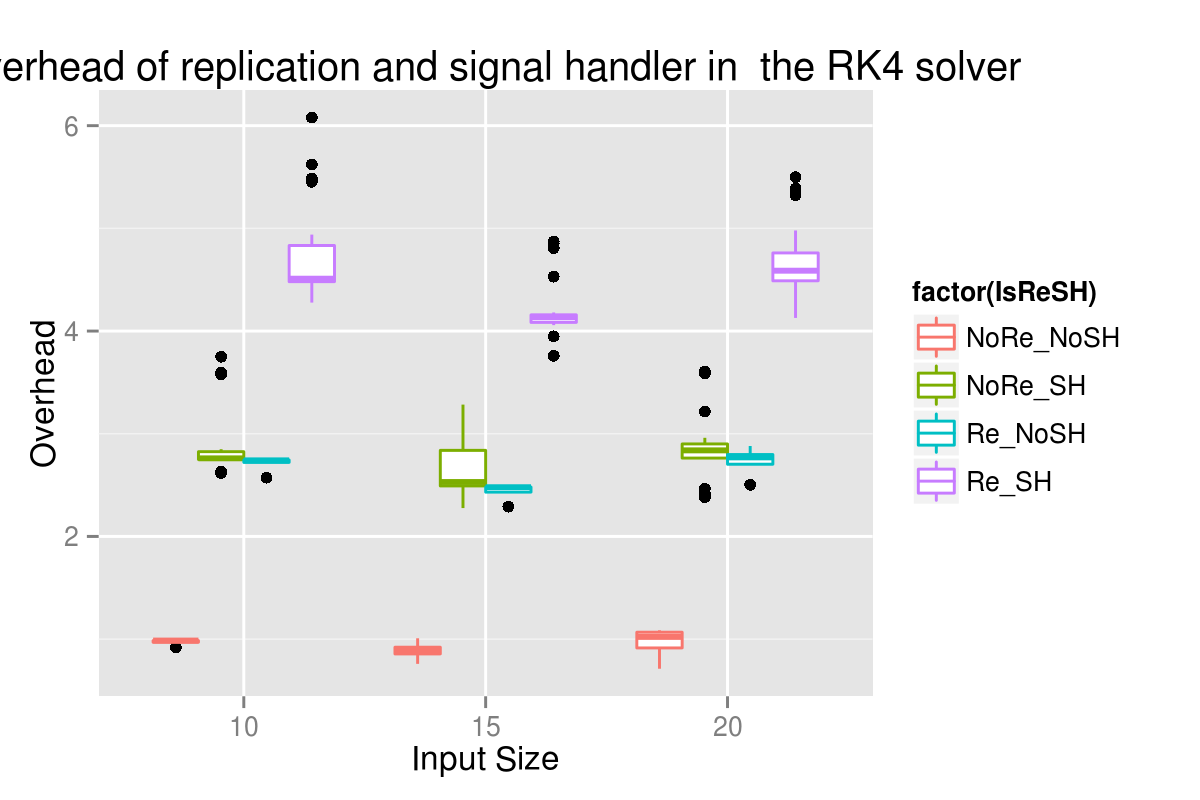
\includegraphics[width=1.00\columnwidth]{figs/4_1_2_Exp2_Overhead_Inputsize.png}
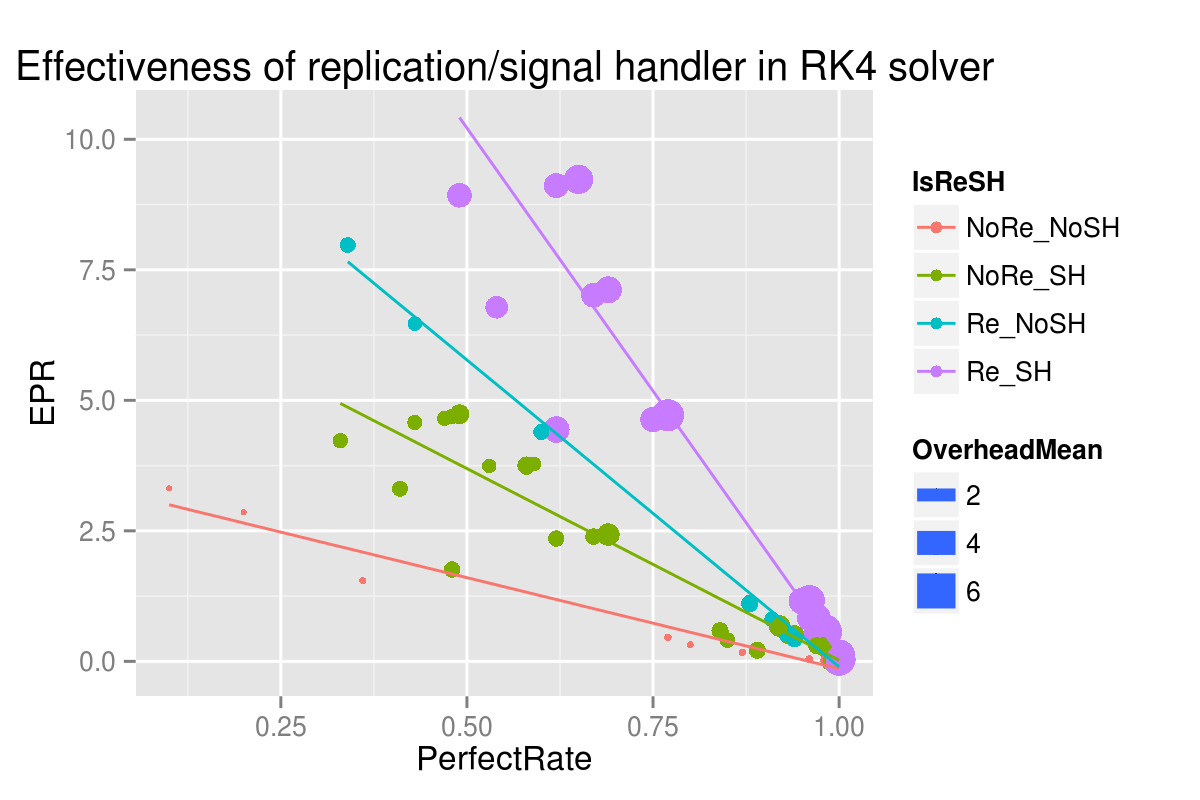
\includegraphics[width=1.00\columnwidth]{figs/4_1_2_Exp2_Effectiveness.png}
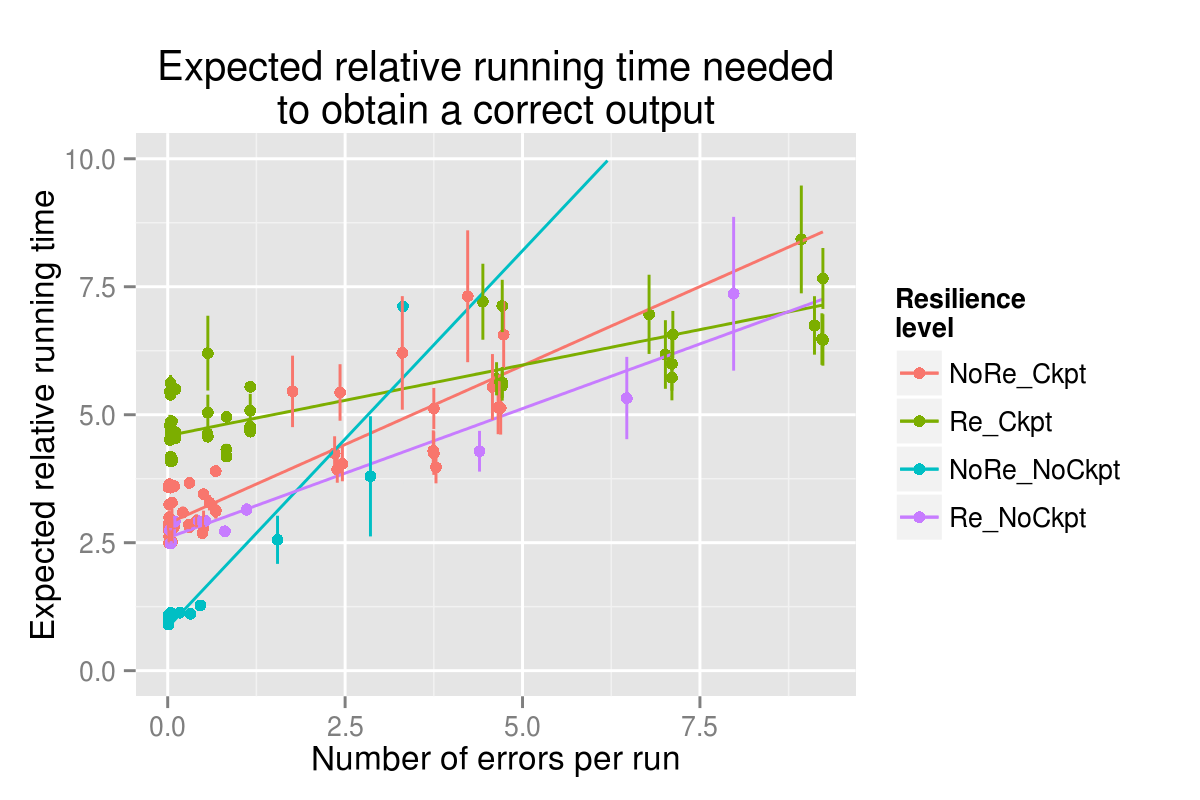
\includegraphics[width=1.00\columnwidth]{figs/4_1_2_Exp2_Expected_Running_Time_Needed.png}
\caption{Overhead and effectiveness of the pointer protection techniques for the ODE solver}
\label{fig:rk4_eff_ovhd}
\end{figure}

Errors that do not cause the application to access an invalid memory location are detected by replicating key pointers and loop iteration variables.
The Hattrick application uses a high-accuracy ODE solver that is capable of estimating errors and detecting and reducing errors to a certain level adaptively.
Therefore we would only focus on the application's vulnerability to pointer and index corruptions.
Replicating critical variables (pointers and indices) and leveraging Byzantine fault tolerance and correcting those pointers and indices during run-time would raise the applications' resistance to soft errors \sui{and increase the chance this application would output correct results.}

\sui{Unlike the numerical and FFT routines used in the other two applications, the ODE solver has an stepping function called on the evaluation(s) of each integration step (GSL performs two evaluations per timestep in order to estimate integration error and perform adaptive step size control), which is called much more frequently, on the magnitude of millions of times during the lifetime of the application. Contrarily, the linear algebra routines are only called less than a hundred times during the execution of Lasso with a 10x input, and the FFT routines are called only several hundred times during the execution of DRC with a 30x input. Both are moderate-sized inputs in our experiments.}

\greg{Need to explain why we only do this for Hattrick.} \sui{The checkpointing scheme used here has overhead of having to set signal handlers and perform up-to-date checksum computation of critical data structures. The more often the routines are called, the more frequent the critical data structures need be kept up-to-date, therefore this overhead is larger (non-trivial compated to that for FFT and linear algebra) for a frequently called routine like the integrator. This overhead makes the fault tolerance technique less efficient as it was in linear algebra and FFT routines, bringing it to the same ballpark as the expensive pointer replciation technique. Although it is possible to reduce the frequency of updating the checkpoints, it would also reduce the effectiveness of this method sharply.}

\sui{
The other reason is, pointer replication performs a better job at maintaining the chance the routine generates correct results (See figure \ref{fig:rk4_eff_ovhd}). This would lower the expected cost the user would have to pay to get the correct result despite the overhead. The method of computing this expected running time is described in greater detail in section \ref{sec:eval:perf}'s Markov Model. From \ref{fig:rk4_eff_ovhd} one could see the ratio of perfect runs out of all runs (that are completed or incomplete) and the number of faults per run forms an almost linear relationship. The linear regression model is used to evaluate the position of the guide points needed for the following experiments.
} 

\sui{Refer to Figure \ref{fig:rk4_eff_ovhd} one could see the number of expected running time of different configurations if one wants to get a correct output from the application in a faulty environments. As the number of faults injected per run increases, the expected running time of the original, non-fault-tolerant application increases at a much faster rate than the other fault-tolerant counterparts. In real life scientific applications that run much longer, it's likely that a fault could hit the application several times before it completes. In such situations, the replication-only resilience technology produces the least expected number of runs needed to get a correct answer.}

To determine a replication strategy we have to determine which variables to replicate and how many replicas to use for replicating them. The following two subsections would be focused on these problems.
\greg{The report spends a lot of space talking about this but in the end the conclusion is that we just a pick a few options and evaluate them experimentally. How much space should we devote to this discussion.}

Experiment 2: Measure the effectiveness and performance costs of replication. Need to explain why we don't use it for Lasso and DRC.

\subsection{Recovery via Checkpoint-Restart}
\label{sec:res_tech:cr}

When errors are detected we employ a recovery method based on checkpoint-restart.
At the start of each routine the state of all inputs is recorded and an error correcting code is used to ensure that the contents of this backup copy are not corrupted.
Further, we use the \texttt{sigsetjmp} routine to record the application's execution state at the routine's start.
If an error is detected during the routine \texttt{siglongjmp} is used to return the application's execution back to the start of the routine (this function unrolls function calls as needed and reloads the process counter and register state).
The recovery procedure then resets the routine's inputs from their backed-up copies, overwriting any changes or corruptions that may have occurred during the routine's execution, and restarts its execution.
%A combination of \texttt{siglongjmp} and \texttt{sigsetjmp} are used to recover from segmentation faults. The overhead of this API call is having to copy the processor state into memory, therefore installing them between computation-intensive method calls adds to negligible performance degradation.

The backup copy of routine inputs is protected via a block-checksum-based data correction mechanism.
By treating the input array as a matrix and comparing row sums and column sums of the submatrices of that matrix, we are able to detect the existence of errors and fix a fraction of the errors.
The protection mechanism has the following parameters:
\begin{itemize}
\item{\texttt{N}, the size of the error correcting sum block.}
\item{\texttt{ECC\_ECC}, whether or not the error correcting code itself should be corrected.}
\end{itemize}
This mechanism is able to correct up to $1/{n^2}$ of the elements in the input array.
\greg{Which code is being used here? You just say that it is based on block-checksums}.

Experiment 1: Measure the cost of setjmp and longjmp in our routines as the input sizes vary
Experiment 2: Measure the cost of input backup and input recovery in our routines as the input sizes vary

\section{Evaluation of Resilience Methodology}
\label{sec:eval}

\greg{This is the section where we put all the pieces together and present the experimental results on full applications. We should describe our main use-case here: user wants to achieve a given accuracy with a given probability and we configure the algorithm to provide this at the lowest cost. QUESTION: how do we pick the parameters of each resilience technique? Which metric is being optimized?} \sui{Using the choices of those parameters derived from the experiments we have already performed (treat it as a ``training set'') and use those choices on some new experiment configurations (treat as ``test set''), and see what is the probability that those choices could satisfy the users' experiments.}

\subsection{Performance Impact}
\label{sec:eval:perf}

Show the Markov model that describes our rollback scheme.

\sui{When a user wants to run an application under a faulty environment and obtain correct results, s/he would have to expect to run a part of this application multiple times in case the application aborts due to memory access errors or return useless incorrect results. The user might want to have the application return to a certain checkpoint, or restart the entire application should any unrecoverable occurs. The cost of rollback, and the chance of each type of errors occurs at a different rate. The Markov model comes into play here with its capability to capture all these parameters of experiments we have already run and predict the running time of the applications at configurations not experimented with.}


Experiment 1: Measure the slowdown of each application at the optimal configuration
Experiment 2: Measure the rate of aborts due to algorithmic errors, segfaults and redundant copy mismatches (separate the causes)

\subsection{Result Accuracy}
\label{sec:eval:acc}

Experiment: Measure the accuracy of the results produced in completed runs, including error bars on the variability of the errors

\subsection{Overall Evaluation}
\label{sec:eval:overall}

Experiment: Final graph that shows slowdown for each desired probability of perfect results.

\section{Summary}
\label{sec:summary}

\bibliographystyle{abbrv}
\bibliography{bibs}

\end{document}
